\documentclass[preprint]{elsarticle}

\usepackage{amssymb}
\usepackage{amsmath}
\usepackage{amsfonts}
%\usepackage{cite}
%\usepackage{graphics}
%\usepackage{epsf}
%\usepackage{psfig}
%\usepackage{float}
\usepackage{graphicx}
\usepackage{epstopdf}
%\usepackage[small]{caption2}
%\usepackage{bm}%
%\usepackage{multirow}
%\usepackage{subfigure}
%\usepackage{wrapfig}
%\usepackage{color}
%\usepackage{dsfont}
%\usepackage{amsthm}
%\usepackage{algorithm}
%\usepackage{subfigure}
\usepackage{subcaption}

\graphicspath{{../}}

%\newtheorem{theorem}{Theorem}
%\newtheorem{corollary}[theorem]{Corollary}
%\newtheorem{lemma}[theorem]{Lemma}
%\newtheorem{observation}[theorem]{Observation}
%\newtheorem{proposition}[theorem]{Proposition}
%\newtheorem{definition}[theorem]{Definition}
%\newtheorem{claim}[theorem]{Claim}
%\newtheorem{fact}[theorem]{Fact}
%\newtheorem{assumption}[theorem]{Assumption}
%%\newtheorem{example}[theorem]{Example}
% \newtheorem{remark}[theorem]{Remark}

\journal{Computers \& Chemical Engineering}
 
\begin{document}

\begin{frontmatter}

\title{Parsimonious Representation of Nonlinear Dynamical Systems using Diffusion Maps: A Chemotaxis Case Study}

\author[princeton]{Carmeline~J.~Dsilva\corref{cor1}}
\ead{cdsilva@princeton.edu}
%
\author[technion]{Ronen~Talmon}
\ead{ ronen@ee.technion.ac.il}
%
\author[yale]{Ronald R. Coifman}
\ead{coifman@math.yale.edu}
%
\author[princeton, princetonpacm]{Ioannis~G.~Kevrekidis \corref{cor1}}
\ead{yannis@princeton.edu}
%
\address[princeton]{Department of Chemical and Biological Engineering, Princeton University, Princeton, NJ, 08540, USA}
\address[technion]{Technion - Israel Institute of Technology, Haifa, 3200003, Israel}
\address[yale]{Department of Mathematics, Yale University, New Haven, CT, 06520, USA}
\address[princetonpacm]{Program in Applied and Computational Mathematics, Princeton University, Princeton, NJ, 08540, USA}
%
\cortext[cor1]{Corresponding author}


\begin{abstract}

TODO
\end{abstract}

%\sloppy

\begin{keyword}
TODO
\end{keyword}

\end{frontmatter}


\section{Introduction}


\begin{itemize}

\item
Data driven analysis methods, and in particular, manifold learning, can do many things (dimensionality reduction, reduction in dynamical systems, etc). 

\item
Manifold learning constructs parameterization of the data through the spectral analysis of a Laplace operator.

\item
Initially it was used almost exclusively for toy examples/synthetic data (``these people suck").

\item
Only recently, has it been applied to real (experimental/simulation) data, and this was possible due to advances in observers (data representation) and metrics (``we are awesome"). 

\item
However, a major limitation (of spectral methods based on a Laplace operator) is identifying the true principal components.

\item
In this paper, we propose an algorithm to automatically identify those principal components using locally linear regression.

\item
All of these considerations (recently developed plus what we propose here) provide a data analysis pipeline. We show that this pipeline can successfully analyze data from a complex stochastic dynamical system originated from the study of cellular dynamics (chemotaxis).

\end{itemize}

\section{Issues in Manifold Learning/Diffusion maps}

\subsection{Diffusion maps}

\subsection{Observers}

\begin{itemize}
\item Physical examples (e.g., $\alpha$-carbons for molecules)
\item Amit's bispectrum
\item Scattering transform
\item Cite PNAS, stating that the histograms are good since they linearize any noise. 
\end{itemize}

\subsection{Metric}

\begin{itemize}
\item Euclidean (not good, especially for histograms)
\item Mahalanobis (good, cite PNAS, since it noise robust)
\item Here we use EMD since it is multiscale.
\item Emphasize stability and regularity issues.
\end{itemize}

\section{Identifying the Principal Components}

\begin{itemize}
\item Discuss the issues: harmonics
\item Give simple example (Laplacian on strip)
\end{itemize}

\subsection{Algorithm: Local Linear Regression}

Given the eigenvectors $\phi_1, \phi_2, \dots, \phi_{n-1} \in \mathbb{R}^n$, we would like to automatically deduce which ones are harmonics/functions of another. 
%
To accomplish this, we will fit a function $f(\phi_1, \dots, \phi_k)$ to $\phi_{k+1}$. 
%
If the resulting fit is good/accurate, then $\phi_{k+1}$ is most likely a harmonic of $\phi_1, \dots, \phi_k$. 

We will use a local linear function 
\begin{equation}
f_{k+1}(\phi_1, \dots, \phi_k) = a_0 + a_1 \phi_1 + \dots + a_k \phi_k
\end{equation}
where the coefficients $a_0, \dots, a_k$ are functions of $\phi_1, \dots, \phi_k$. 


To find these coefficients, we want to minimize the local weighted sum of squares
\begin{equation} \label{eq:opt_problem}
\sum_{i=1}^n w_i(x) (\phi_{k+1}(x) - f_{k+1} (\phi_1(x), \dots, \phi_{k}(x))
\end{equation}
where $w$ is a weighting function.
%
We will use
%
\begin{itemize}
\item $w_i(x) = \exp \left( - \frac{\|\Phi_{k}(x) - \Phi_{k} (x_i) \|^2}{\epsilon^2} \right)$, where $\Phi_k(x) = \begin{bmatrix}
\phi_1(x) \\
\vdots \\
\phi_k(x)
\end{bmatrix} $
\item $\epsilon = M / 3$, where $M$ is the median of the pairwise distances between $\Phi_{k}(x)$
\end{itemize}

Let $\hat{f}_{k+1}(\phi_1(x_i), \dots, \phi_k(x_i))$ denote the minimum achieved in \eqref{eq:opt_problem}, when the minimization is performed over $x_j$ with $j \ne i$. 
%
We then define the leave-one-out- cross-validation error as
\begin{equation}
r_{k+1} = \sum_{i=1}^n \left( \phi_{k+1} (x_i) - \hat{f}_{k+1}(\phi_1(x_i), \dots, \phi_k(x_i)) \right)^2
\end{equation}
%
A small value of $r_{k+1}$ means that $\phi_{k+1}$ can be accurately approximated from $\phi_1, \dots, \phi_k$, and is therefore a harmonic of a previous mode.
%
A large value of $r_{k+1}$ indicates that $\phi_{k+1}$ parameterizes a new direction in the data.

\subsection{Eigenvalues to Quantify Dimensions}

The eigenvalues of the Laplacian with Neumann boundary conditions on a $d$-dimensional rectangular domain are given by
\begin{equation}
\mu_{k,l} = \frac{k^2 \pi^2}{L_l^2}
\end{equation}
for $k=1, 2, \dots$ and $l=1, 2, \dots, d$, and $L_l$ is the length of the domain along the $l^{th}$ dimension. 
%
These eigenvalues are related to the eigenvalues we compute in diffusion maps by 
\begin{equation}
\lambda_{k,l} = e^{-\mu_{k,l} t} = e^{-\frac{k^2 \pi^2}{L_l^2} t}
\end{equation}
%
Therefore, 
\begin{equation}
\sqrt{\frac{\log(\lambda_{1,l_1})}{\log(\lambda_{1,l_2})}} = 
\frac{L_{l_2}}{L_{l_1}}
\end{equation}
and so looking at the ratio of the log of the eigenvalues (modulo harmonics) should inform us as to the lengths of the different directions in the manifold. 

\subsection{Illustrative Examples}


\subsubsection{Swiss Roll}

\begin{figure}
%
\begin{subfigure}{0.45\textwidth}
\centering
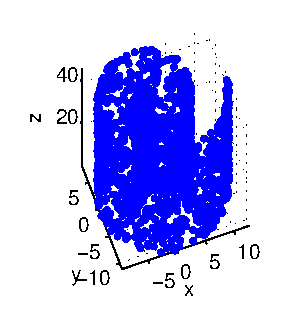
\includegraphics[height=1.5in]{swissroll1}\\
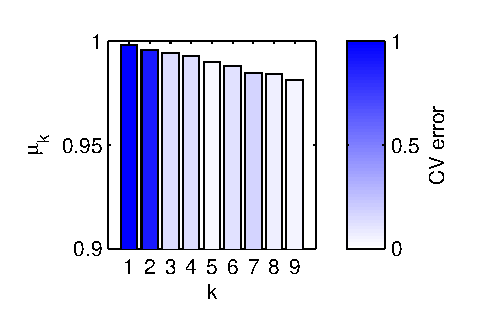
\includegraphics[height=1.5in]{swissroll1_evals}\\
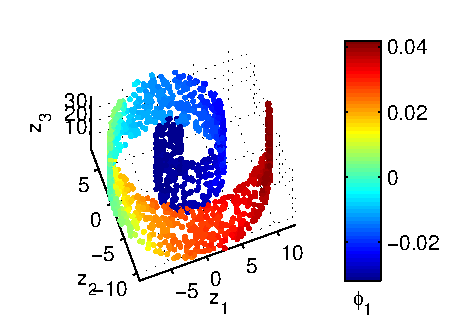
\includegraphics[height=1.5in]{swissroll1_color1}\\
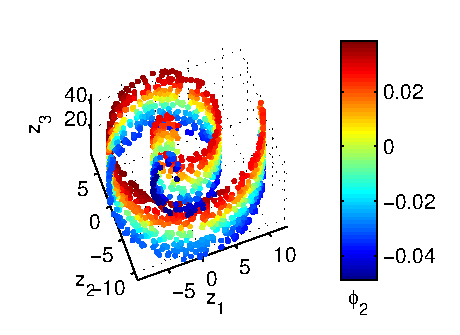
\includegraphics[height=1.5in]{swissroll1_color2}
\caption{}
\end{subfigure}
\hfill
\begin{subfigure}{0.45\textwidth}
\centering
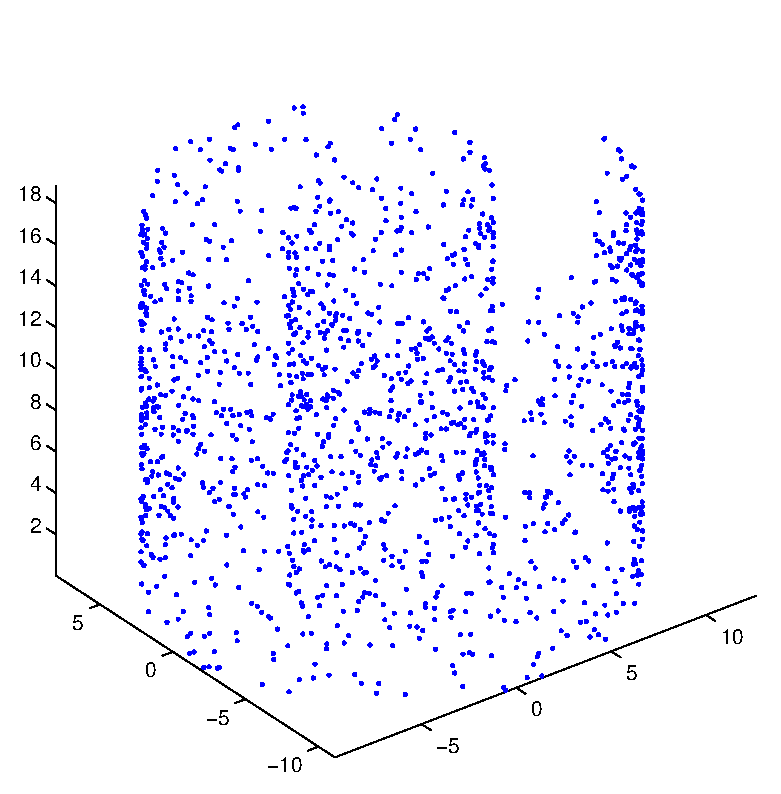
\includegraphics[height=1.5in]{swissroll2} \\
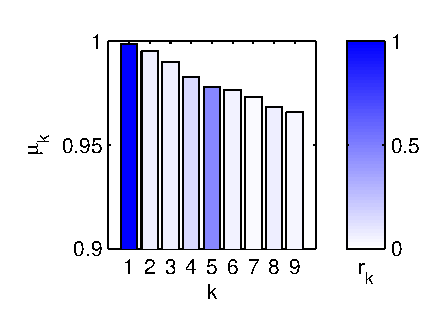
\includegraphics[height=1.5in]{swissroll2_evals} \\
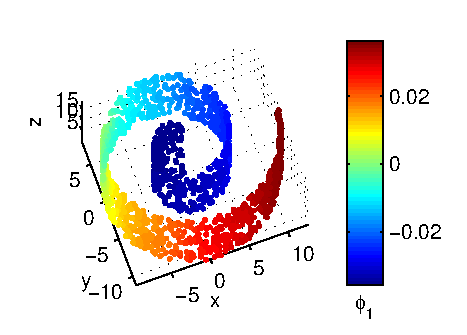
\includegraphics[height=1.5in]{swissroll2_color1}\\
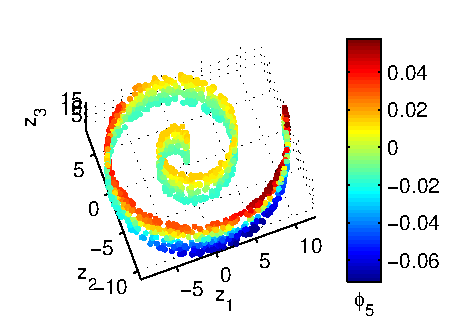
\includegraphics[height=1.5in]{swissroll2_color2}
\caption{}
\end{subfigure}
%
\caption{}
\end{figure}

%For first case: $\lambda_1 = 0.9982$, $\lambda_2 = 0.9959$

%For second case: $\lambda_1 = 0.9977$, $\lambda_5 = 0.9652$.

\subsubsection{Torus}


\begin{figure}[t]
%
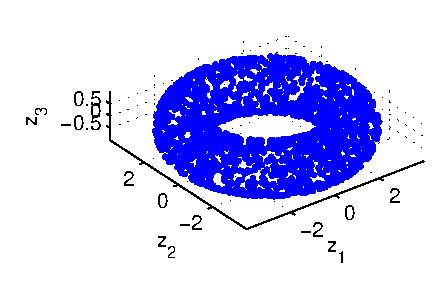
\includegraphics[width=2.5in]{torus1}
\hfill
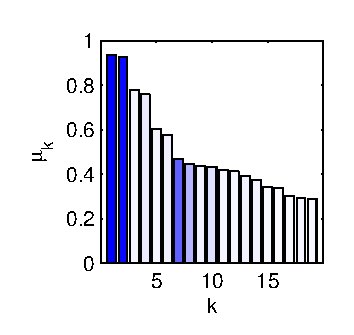
\includegraphics[height=1.5in]{torus1_evals}\\
%
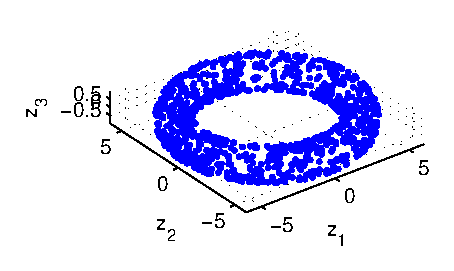
\includegraphics[width=2.5in]{torus2}
\hfill
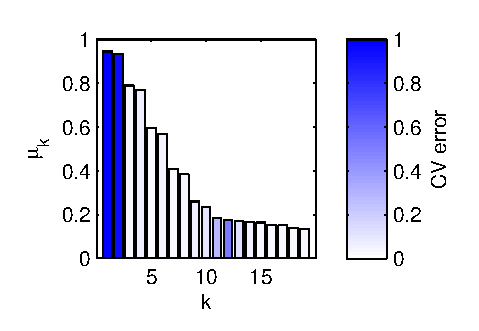
\includegraphics[height=1.5in]{torus2_evals}\\
%
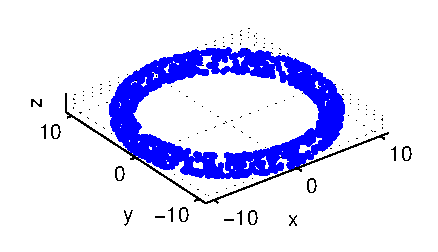
\includegraphics[width=2.5in]{torus3}
\hfill
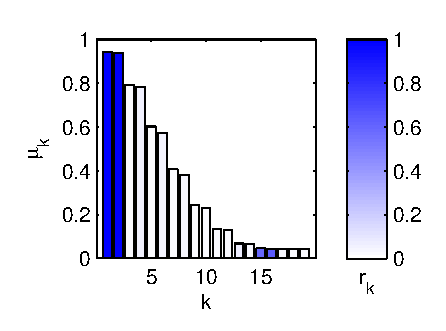
\includegraphics[height=1.5in]{torus3_evals}
%
\caption{}
\end{figure}


\section{Chemotaxis: a case study}

Often, systems which are stochastic and noisy on the microscale exhibit coherent dynamics on the macroscale which are governed by only a few parameters.
%
For example, fluid flow, which can be described via the position and velocity of every fluid particle, is modeled at the macroscale using the Navier-Stokes equations.
%
However, in general, this mapping from microscale to macroscale is not always obvious.
%
We would like to extract a parameterization of data collected at the microscale which is consistent with the macroscopic behavior, without any {\em a priori} knowledge of the appropriate microscopic or macroscopic model.

In this letter, we will demonstrate how this goal can be achieved through a data-driven method based on geometric analysis and manifold learning. 
%
Specifically, we aim to emphasize two particular aspects of manifold learning from a dynamical systems' point of view: (a) choosing the appropriate observers, especially in presence of stochastic dynamics, and (b) selecting an appropriate metric for comparison \cite{mallat2012group}. 
%
We will show that both are essential for data-driven algorithms to successfully uncover the underlying system dynamics. 

We will illustrate these points using a model problem which arises in studies of cellular chemotaxis \cite{othmer2000diffusion}.
%
In this example, the macroscopic dynamics vary depending on the value of a single system parameter.
%
We will demonstrate how we can use diffusion maps \cite{coifman2005geometric}, a manifold learning technique, to {\em automatically} detect changes in the system's macroscopic dynamics from microscale data.
%
This case study exhibits several key points which allow us to demonstrate the strength of our approach.
%
First, this system has random microscopic behavior with smooth macroscopic dynamics governed by a single parameter which determines the regime/mode of the system. 
%
Second, it consists of an ensemble of individual stochastic particles which must be described using the appropriate observers.
%
Third, it has an analytic macroscopic description, which serves as a ground truth and will allow us to verify our results which are obtained in an unsupervised manner.
%
We will show that manifold learning algorithms based on statistical observers and with the appropriate affinity metric between pairs of observations uncovers a parameterization of the microscopic data which is consistent with the macroscopic model.
%
Furthermore, these data-driven methods allow us to detect changes in dynamical behavior resulting from changes in the system parameters. 

%The remainder of this letter is organized as follows. 
%
%We begin by describing the chemotaxis problem, the illustrative example used to demonstrate the methodologies.
%%
%We present the stochastic microscopic model, and use diffusion maps, a nonlinear dimensionality reduction technique, to analyze microscopic simulation results.
%%
%We show that the governing macroscopic variables can be recovered, provided that the appropriate observers and distance metric are used.
%%
%We then describe how, for this example, the microscopic model gives rise to a compact macroscopic description governed by a single parameter, and show that the diffusion maps results are consistent with this macroscopic description. 
%%
%Finally, we demonstrate that diffusion maps can also identify the relative importance of system variables in different parameter regimes, and detect changes in macroscopic dynamical behavior.

%\section{Problem formulation}

%\subsection{Chemotaxis ``story''} 

Biological cells are one common example of a system where microscopic entities work together and exhibit coherent macroscopic dynamics, in order to accomplish tasks such as finding food or navigating away from toxins.
%
The cellular dynamics are often governed by extracellular sensed signals; this movement is known as chemotaxis. 
%
Several microscopic models have been proposed to describe chemotaxis dynamics \cite{othmer1988models, codling2008random}.
%
We will analyze one such model described by a one-dimensional velocity jump process \cite{othmer2000diffusion}.
%
In this model, each cell is initialized with a position and a velocity on a line, and the dynamics of each cell are governed by a stochastic process.
%
At random times, a cell will ``turn around'' and switch the direction of its velocity (this turning is controlled by extracellular signals). 
%
%We will analyze the dynamics of collections of such cells/particles. 

%\subsection{Stochastic particles}

The microscopic model consists of a collection of $N$ particles whose states are defined by their positions and velocities. 
%
Let $x_i(t)$ and $v_i(t)$ denote the position and velocity, respectively, of particle $i$ at time $t$.
%
The velocity of each particle is either $\pm s$, where $s$ is a (fixed) speed. 
%
We initialize the particles such that
\begin{equation}\label{eqn:system}
\begin{aligned}
x_i(0) & = 0 \\
\mathbb{P} \{ v_i(0) = +s \} & = p
\end{aligned}
\end{equation}
where $0 < p < 1$ is the probability of a particle initially moving to the right.
%
The velocity of each particle randomly switches between $\pm s$ following an (independent) Poisson process with rate $\lambda$.
%
We would like to note that we have chosen a very specific one-parameter family of initial conditions, which lead to simple dynamics and straightforward illustration of our main points.
%
More complex initial conditions could easily be chosen. 

This particular example has a known analytic macroscopic equation that governs the overall system behavior.
%
For a large collection of particles ($N \rightarrow \infty$), the system can be described by the probability density of the particles.
%
Let $\rho(x, t)$ denote the probability density of the particles, and let $\rho^-(x, t)$ and $\rho^+(x, t)$ denote the densities of the particles moving towards the positive and negative axis directions, respectively.
%
It can be shown that, as $N \rightarrow \infty$, the densities obey the following set of partial differential equations (PDEs) \cite{othmer2000diffusion}:
\begin{equation} \label{eqn:coupled_pdes}
\begin{aligned}
\frac{\partial \rho^+}{\partial t} + s \frac{\partial \rho^+}{\partial x} & = -\lambda \rho^+ +\lambda \rho^- \\
\frac{\partial \rho^-}{\partial t} - s \frac{\partial \rho^-}{\partial x} & = \lambda \rho^+ -\lambda \rho^- 
\end{aligned}
\end{equation}
%
Alternatively, \eqref{eqn:coupled_pdes} can be rewritten as one, second--order PDE:
\begin{equation} \label{eq:second_order_pde}
\frac{\partial^2 \rho}{\partial t^2} + 2 \lambda \frac{\partial \rho}{\partial t} = s^2 \frac{\partial ^2 \rho}{\partial x^2}
\end{equation}
%
%We assume that $s^2/\lambda = D$ is constant, so that the dynamics of the probability density are governed by a {\em single} parameter $\lambda$.
%
From \eqref{eq:second_order_pde}, we see that, for fixed values of $\lambda$ and $s$, the macroscopic state of the system (the probability density of the particles) is a function of two independent variables: $p$, which controls the initial distribution of the particles, and $t$, the time. 
%
This implies that for fixed $\lambda$ and $s$, the {\em microscopic} data in a high-dimensional ambient space (e.g., the positions of all $N$ particles) should lie on a two-dimensional manifold parameterized by $p$ and $t$, 
and uncovering the low-dimensional structure of the microscopic data reveals this manifold.

We consider two asymptotic regimes of simulation.
%
When $\lambda \rightarrow 0$, the right-hand side of \eqref{eqn:coupled_pdes} tends to 0, and \eqref{eqn:coupled_pdes} becomes two uncoupled wave equations,
\begin{equation}
\begin{aligned}
\frac{\partial \rho^+}{\partial t} + s \frac{\partial \rho^+}{\partial x} & = 0 \\
\frac{\partial \rho^-}{\partial t} - s \frac{\partial \rho^-}{\partial x} & = 0.
\end{aligned}
\end{equation}
%alternatively, \eqref{eq:second_order_pde} becomes the second order wave equation,
%\begin{equation}
%\frac{\partial^2 \rho}{\partial t^2} = s^2 \frac{\partial ^2 \rho}{\partial x^2}.
%\end{equation}

%Dividing \eqref{eq:second_order_pde} by $\lambda > 0$ yields
%\[
%\frac{1}{\lambda} \frac{\partial^2 \rho}{\partial t^2} + 2 \frac{\partial \rho}{\partial t} = D \frac{\partial ^2 \rho}{\partial x^2}
%\]
When $\lambda \rightarrow \infty$, \eqref{eq:second_order_pde} approaches the heat equation,
\begin{equation}
2 \frac{\partial \rho}{\partial t} = D \frac{\partial ^2 \rho}{\partial x^2}.
\end{equation}
%
%Two variables determine the macroscopic state of the system: the initial distribution, which is controlled by a single parameter $p$, and the time, $t$.
%
The above analysis shows that the initial distribution of velocities of the particles (determined by $p$ in the microscopic simulations) plays a very different role depending on the value of $\lambda$.
%
When $\lambda \rightarrow 0$, the dynamics are described by two wave equations, and the initial distribution persists throughout the trajectory.
%
When $\lambda \rightarrow \infty$, the dynamics are described by one heat equation, and the initial conditions are insignificant -- the velocity distribution quickly equilibrates and we see purely diffusive behavior.

For general dynamical systems, the governing macroscopic variables and asymptotic behavior may not be immediately obvious, and instead need to be inferred from the microscopic data.
%
We expect the simulation data to lie on a low-dimensional manifold which is parameterized by the macroscopic variables.
%
We use diffusion maps \cite{coifman2005geometric}, which is a manifold learning technique, to uncover such low-dimensional structure and to analyze the results of the microscopic chemotaxis simulations.
%
Compared to principal components analysis (PCA) \cite{shlens2005tutorial}, a standard linear technique, diffusion maps provides a parameterization of data which lie on a low-dimensional, (possibly) {\em nonlinear} structure in a high-dimensional space.
%
Diffusion maps is one of many recently introduced manifold learning techniques that could be used to analyzed this data \cite{roweis2000nonlinear, tenenbaum2000global, Belkin2003}.

\begin{figure}[t!]
\begin{subfigure}{6cm}
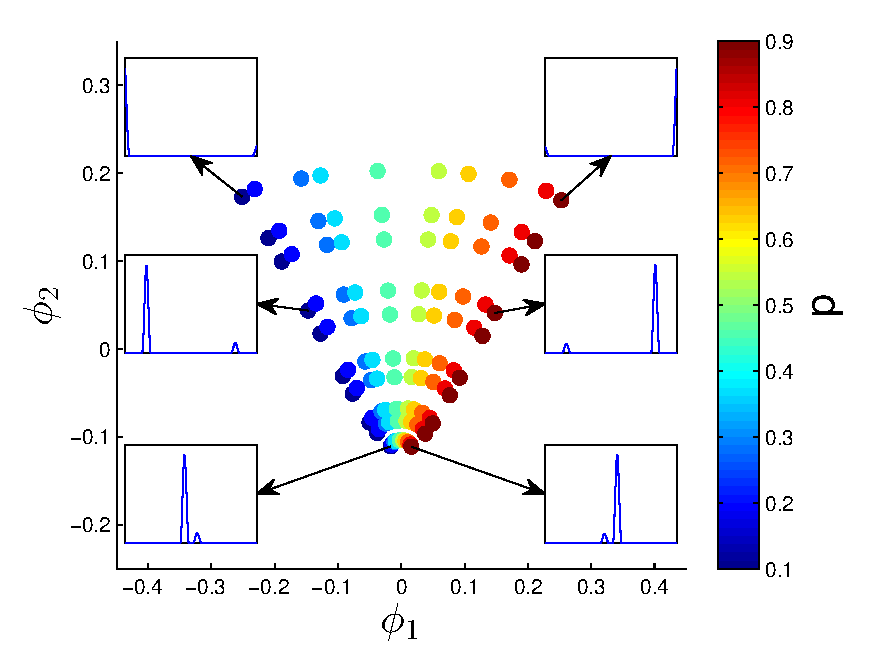
\includegraphics[width=\textwidth]{EMD_withhist_p_1}
\caption{}
\label{subfig:small_lambda_p}
\end{subfigure}
\begin{subfigure}{6cm}
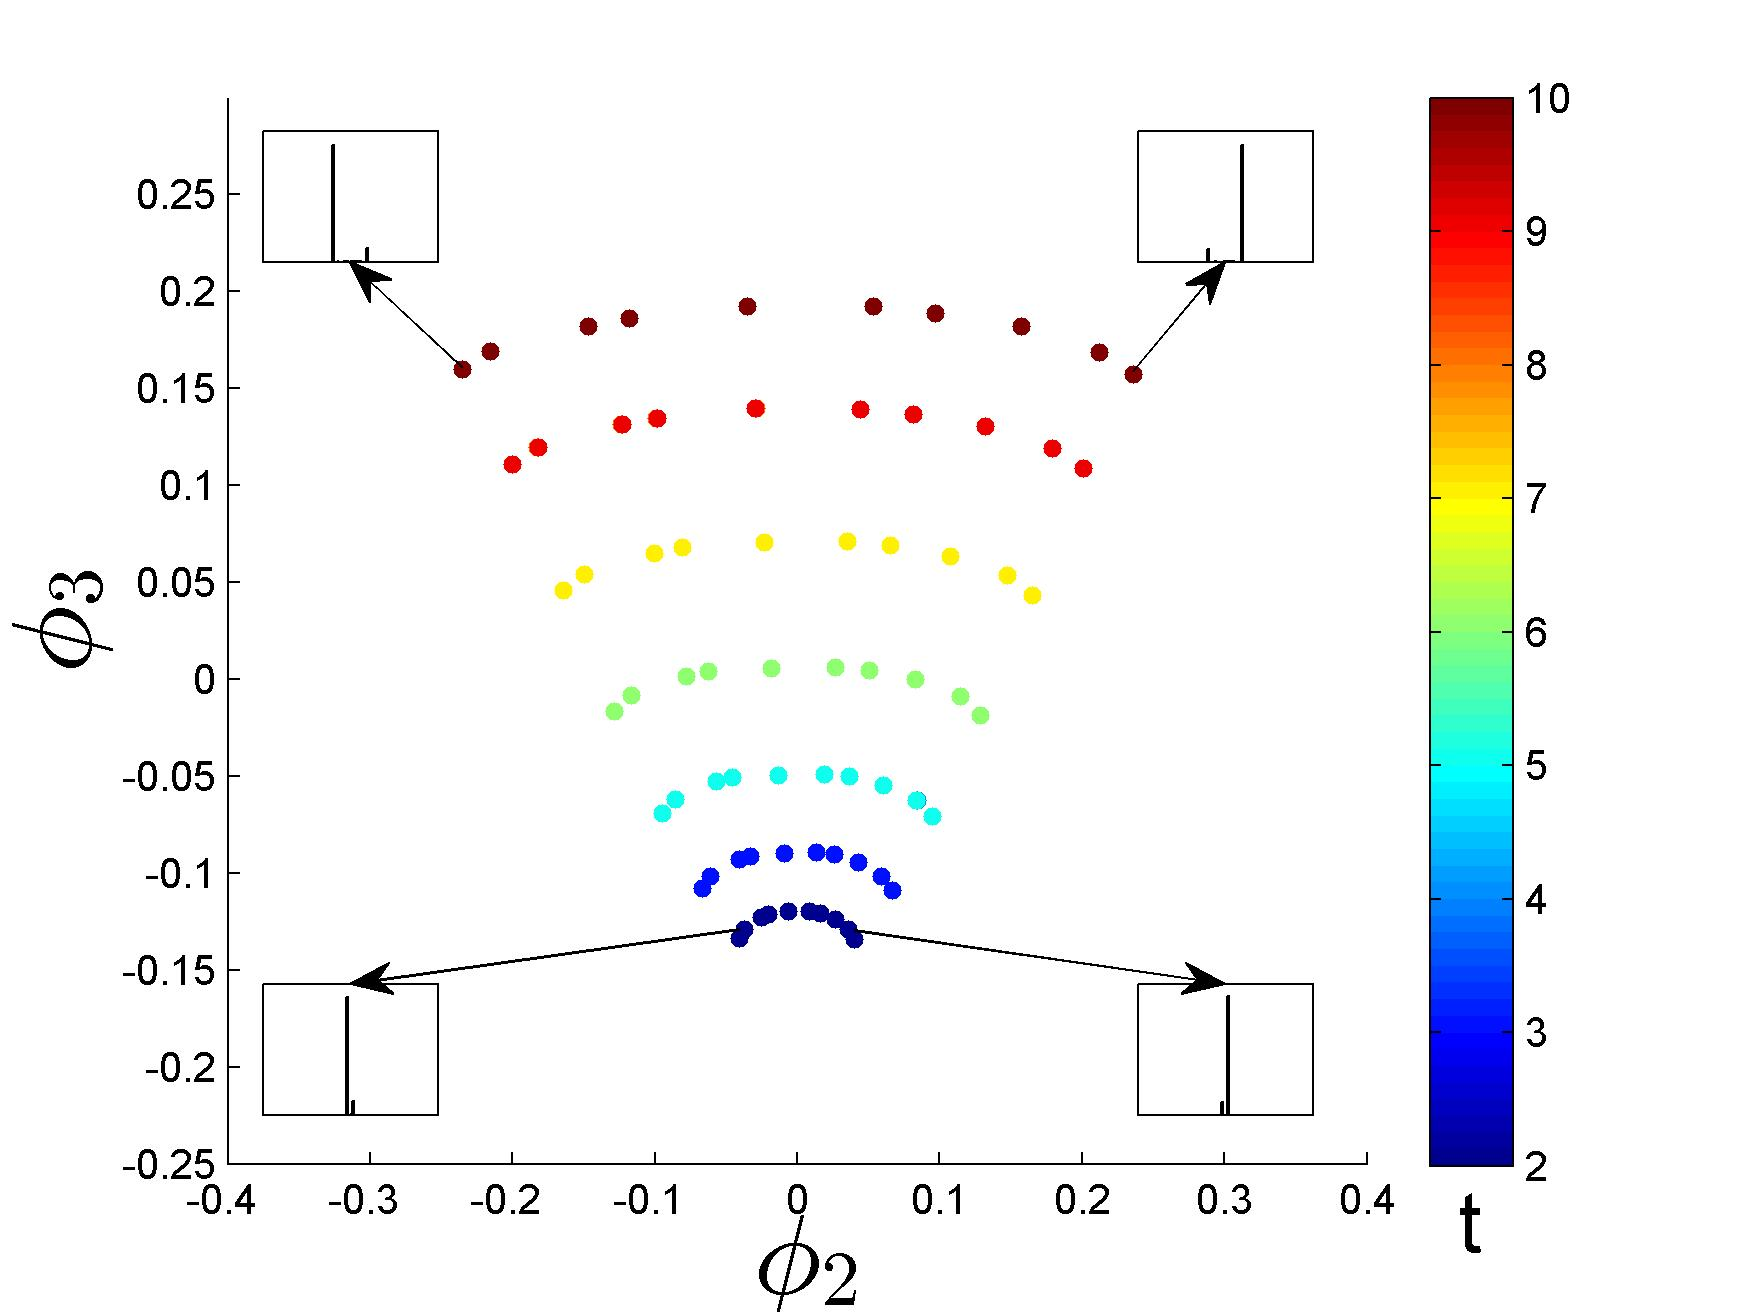
\includegraphics[width=\textwidth]{EMD_withhist_t_1}
\caption{}
\label{subfig:small_lambda_t}
\end{subfigure}
\begin{subfigure}{6cm}
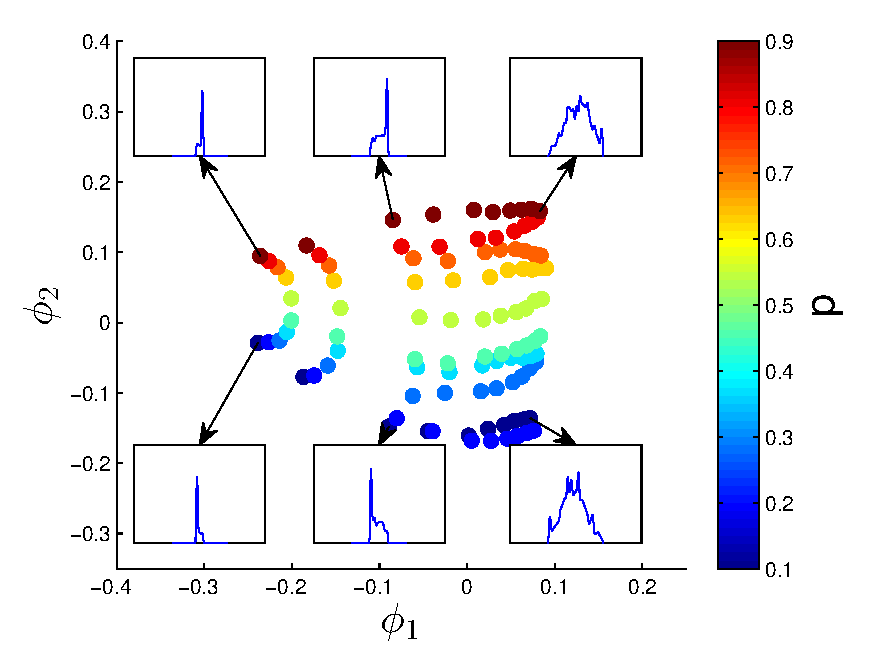
\includegraphics[width=\textwidth]{EMD_withhist_p_400}
\caption{}
\label{subfig:large_lambda_p}
\end{subfigure}
\begin{subfigure}{6cm}
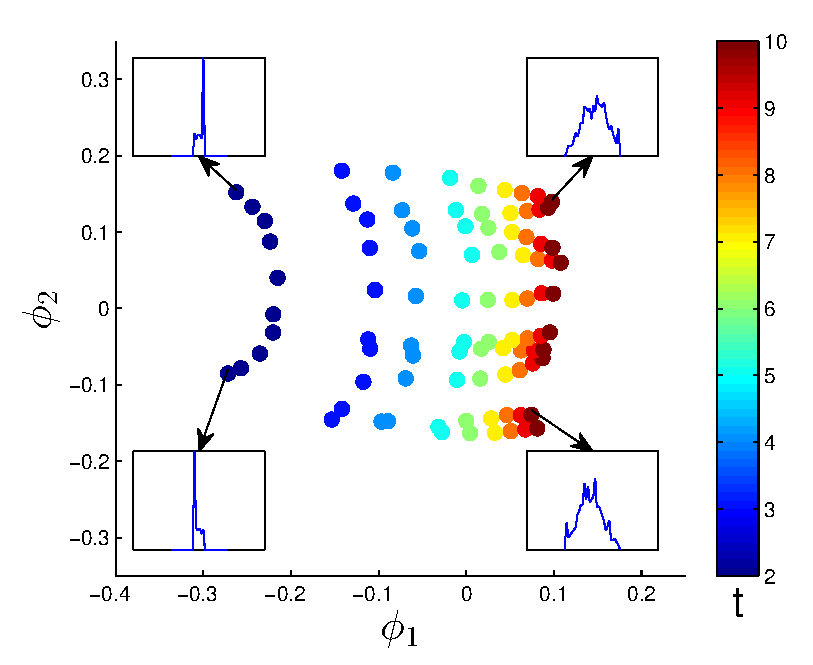
\includegraphics[width=\textwidth]{EMD_withhist_t_400}
\caption{}
\label{subfig:large_lambda_t}
\end{subfigure}
\caption{Diffusion maps embeddings computed from simulation data of the velocity jump process with (a,b) $\lambda=1$, $s=1$, and (c,d) $\lambda=400$, $s=20$.  For each set, we run many simulations, each with $N=1000$ particles.
%
We vary the initial conditions such that $0.1 \le p  \le 0.9$, and allow each simulation to evolve for $10$ time units.
%
We discard the initial portion of each simulation trajectory ($t < 1$), which corresponds to the initial relaxation of the system.
%
The observation $z(i) \in \mathbb{R}^n$ is the histogram of $x_1(i), x_2(i), \dots, x_N(i)$ into $n = 32$ bins.
%
The distances used in the diffusion maps kernel are the earth mover's distances between the histograms of particle positions. The data are colored by (a, c) $p$, the initial probability of a particle moving to the right, and (b, d) $t$, time. Representative histograms are shown for selected data points.}
\label{fig:dmaps_embed_emd}
\end{figure}

In general, manifold learning techniques have two essential components.
%
One is the appropriate {\em observers} of the system. 
%
These observers should be informative as to the state of the system, as well as insensitive to noise in the system. 
%
Two is a {\em distance metric} between the observations that captures a notion of locality: observations which we perceive to be similar should have a small distance. 

Let $z(t) \in \mathbb{R}^n$ denote an $n$-dimensional observation of the system at time $t$. 
%
For the chemotaxis example, we use histograms of the particle positions as observers \cite{talmon2013empirical}. 
%
Histograms are invariant to the indexing of the particles, while retaining the spatial locations of the particles.
%
Instead of the standard Euclidean distance, we use the earth mover's distance (EMD) \cite{rubner2000earth} as the metric between pairs of histograms. 
%
Conceptually, the EMD measures how much ``work'' it takes to transform one probability density into another.
%
It therefore not only considers where the densities are inconsistent, but also how far apart the inconsistencies are.
%
Although the brute-force computation of the EMD is computationally expensive, there has been a plethora of work in developing efficient algorithms for its computation \cite{Pele-eccv2008, Pele-iccv2009}.
%
For the special case of one-dimensional data, the EMD is equivalent to the $L_1$-norm between the cumulative distribution functions \cite{rubner2000perceptual}, which can be estimated from histograms as
\begin{equation}
\| z(i) - z(j) \|_{EMD} \approx \sum_{l=1}^{n} \left| \sum_{k=1}^l z_k(i) - \sum_{k=1}^l z_k(j) \right|
\end{equation}
where the histograms $z(i), z(j)$ are defined on equally-spaced bins in $\mathbb{R}$. 

Assume we are given $m$ observations $z(1), \dots, z(m)$, which lie on a $d$-dimensional, nonlinear manifold, with $d \ll n$. 
%
Our goal is to uncover a $d$-dimensional parameterization of the $m$ observations that respects the underlying manifold geometry.
%
We first construct the matrix $W \in \mathbb{R}^{m \times m}$, with
\begin{equation} \label{eq:W}
W_{ij} = \exp \left( -\frac{\|z(i) - z(j) \|^2}{\epsilon^2} \right), \ i,j=1,\ldots,m
\end{equation}
where $\| \cdot \|$ denotes the appropriate norm for the observations, and $\epsilon$ is a characteristic distance between the observations. 
%
For the chemotaxis example, we use the EMD as the norm, and we take $\epsilon$ to be the median of the pairwise distances between the data points.
%
We then construct the diagonal matrix $D \in \mathbb{R}^{m \times m}$, with $D_{ii} = \sum_j W_{ij}$, and the matrix $A  = D^{-1} W.$
%
The eigenvectors $\phi_0, \phi_1, \dots, \phi_{m-1}$ of $A$ provide the embedding coordinates for the data, such that
$\phi_{j}(i)$ is the $j^{th}$ embedding coordinate for $z(i)$.
%
The ``importance'' of coordinate $\phi_j$ is quantified by the corresponding eigenvalue $\mu_j$, e.g., the relative importance of $\phi_1$ versus $\phi_2$ can be measured by comparing $\mu_1$ and $\mu_2$.
%
We order the eigenvectors such that $|\mu_0| \ge |\mu_1| \ge \dots \ge |\mu_{m-1}|$, and if the data are low-dimensional, we only need to retain a few of the leading eigenvectors to adequately describe the data.
%
Because the matrix $A$ is row-stochastic ($\sum_j A_{ij} = 1$),  $\mu_0 = 1$ and $\phi_0$ is a constant vector which is not used as an embedding coordinate.

Figure~\ref{fig:dmaps_embed_emd} shows the results of analyzing two sets of chemotaxis simulations using diffusion maps. 
%
One set of simulations (Figures~\ref{subfig:small_lambda_p}~and~\ref{subfig:small_lambda_t}) is for a small value of $\lambda$, and the other set (Figures~\ref{subfig:large_lambda_p}~and~\ref{subfig:large_lambda_t}) is for a large value of $\lambda$. 
%
For both sets of simulations, the two macroscopic variables, $p$ and $t$, are well-correlated with the first two diffusion maps coordinates, $\phi_1$ and $\phi_2$. 
%
In both cases, $\phi_1$ is significantly more important than $\phi_2$, as indicated by the separation between the first two eigenvalues (for the small $\lambda$ case, $\mu_1 = 0.5138$, and $\mu_2 = 0.3943$, and for the large $\lambda$ case, $\mu_1 = 0.5543$, and $\mu_2 = 0.3807$).
%
$\phi_1$, the ``more important'' coordinate, is correlated with $p$ for the small $\lambda$ case (Figure~\ref{subfig:small_lambda_p}), and correlated with $t$ for the large $\lambda$ case (Figure~\ref{subfig:large_lambda_t}), indicating that the relative importance of $p$ and $t$ changes in the two simulations;
this is consistent with the analytic macroscopic description. 
%
Furthermore, in the small $\lambda$ regime (wave equation), shown in Figures \ref{subfig:small_lambda_p} and \ref{subfig:small_lambda_t}, the points corresponding to small times are more tightly clustered than the points corresponding to large times.
%
This is in agreement with the macroscopic model: at small times, the particles are more condensed around $x=0$, and it is more difficult to distinguish the particles moving to the left from the particles moving to the right. 
%
On the other hand, at large times, once the particles evolve from the origin, this separation is clear.  
%
For the large $\lambda$ case (heat equation), shown in Figures \ref{subfig:large_lambda_p} and \ref{subfig:large_lambda_t}, we observe that at small times, the initial distribution $p$ is well organized in the embedding in Figure \ref{subfig:large_lambda_p}, as the skew of the velocity distribution can be seen in the initial displacements.
%
On the other hand, for large times, we observe that the initial distribution $p$ is less organized in Figure \ref{subfig:large_lambda_p}, as the velocities have equilibrated and the initial distribution is less detectable in the particle density.
%
Overall, in both cases, we obtain, in an unsupervised data-driven manner, an accurate picture of the macroscopic variables that govern the system dynamics.

%correlations
%small lambda
%Euclidean: 3.3848e-04, -0.1861
%EMD: 0.9000, 0.9807
 %   
%large lambda
%Euclidean: -0.5466, 0.3329
%EMD: 0.9329, 0.9832

To emphasize the importance of using the correct distance metric, we applied diffusion maps to the two sets of simulation data, using the standard Euclidean distance between the histograms to compute the distances in \eqref{eq:W}.
%
There is no appreciable correlation between the embedding coordinates and the macroscopic variables $p$ and $t$ (the correlations between the embedding coordinates and the governing macroscopic variables are all  less than 60\%, with the correlations for the small $\lambda$ case being less than 20\%). 
%
This is due to using an inappropriate metric which does not accurately describe the distances between histograms.
%
In contrast, the correlations between the embedding coordinates and the macroscopic variables when using EMD in the diffusion maps calculation are all greater than 90\%.



\begin{figure}[t] 
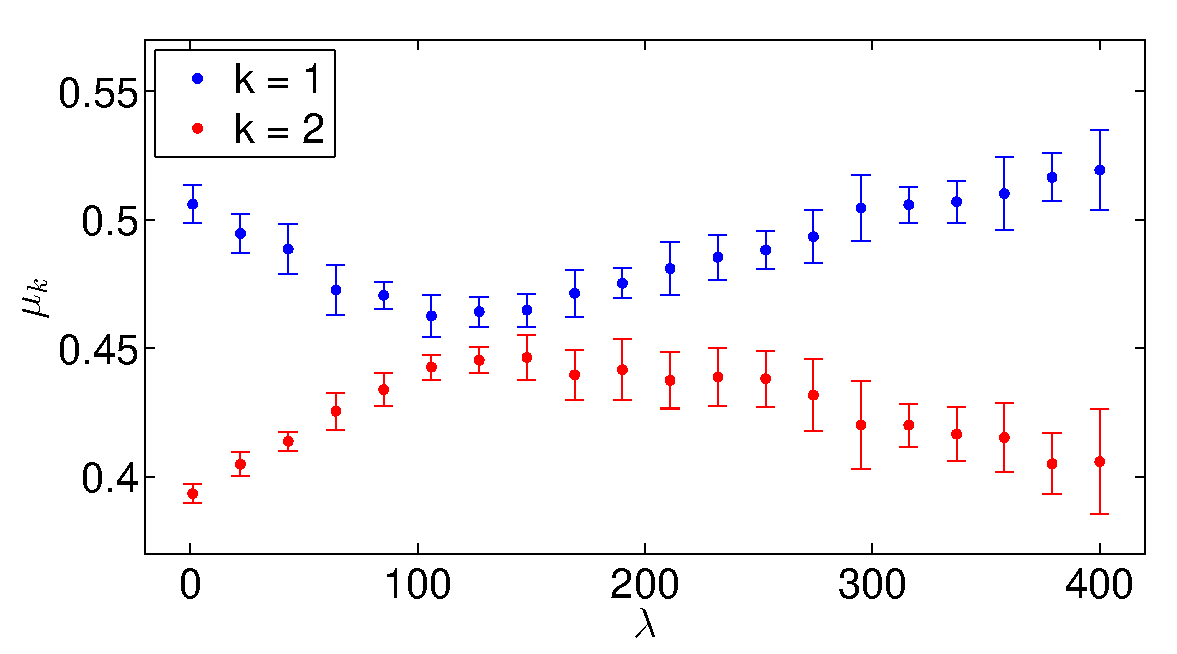
\includegraphics[width=8cm]{detect_change_eigenvalues}
\caption{The first two eigenvalues from diffusion maps as a function of $\lambda$. Each point is averaged over $10$ simulation experiments (as in Figure~\ref{fig:dmaps_embed_emd}, one experiment consists of data collected at varying $p$ and $t$, for a fixed value of $\lambda$), with error bars denoting one standard deviation. 
The convergence of the eigenvalues at $\lambda \approx 125$ indicates switching of the dynamical ``mode''.}
\label{fig:detect_change}
\end{figure}

We have seen that the eigenvalues $\mu_i$, which quantify the importance of each embedding coordinate, reveal the relative importance of the variables which govern the macroscopic dynamics.
%
We can also use these eigenvalues to detect changes in dynamical behavior.
%
We showed that at the two asymptotic regimes ($\lambda \rightarrow 0$ and $\lambda \rightarrow \infty$), there is a gap between the two eigenvalues, as one of the two macroscopic variables is significantly more important to the dynamical behavior.
%
For intermediate $\lambda$ values, we expect the gap between $|\mu_1|$ and $|\mu_2|$ to narrow, with the $\lambda$ value where $|\mu_1| \approx |\mu_2|$ corresponding to the transition between ``wave-like'' and ``heat-like'' behavior. 

To demonstrate this point, we performed a new set of experiments, where we simulated the velocity jump process system over a range of $\lambda$ values. 
% 
Figure~\ref{fig:detect_change} shows the first two diffusion maps eigenvalues, $\mu_1$ and $\mu_2$, computed from these simulations, as a function of $\lambda$.
%
For small $\lambda$ (the wave-equation regime, corresponding to Figures~\ref{subfig:small_lambda_p}~and~\ref{subfig:small_lambda_t}), the two eigenvalues are well-separated, as the first mode (which parameterizes $p$) is significantly more important than the second mode (which parameterizes $t$).
%
At intermediate $\lambda$ values, the eigenvalues come together as the system dynamics change and both $p$ and $t$ are of similar importance.
%
The eigenvalues then separate again at large $\lambda$ (the heat equation regime, corresponding to Figures~\ref{subfig:large_lambda_p}~and~\ref{subfig:large_lambda_t}), where the $t$ effects dominate the dynamics.
%
We can therefore detect changes in dynamical behavior using data-driven techniques, without any knowledge of the governing macroscopic model. 

%\begin{figure}[t]
%\def\figwidth{4.2cm}
%\begin{subfigure}{\figwidth}
%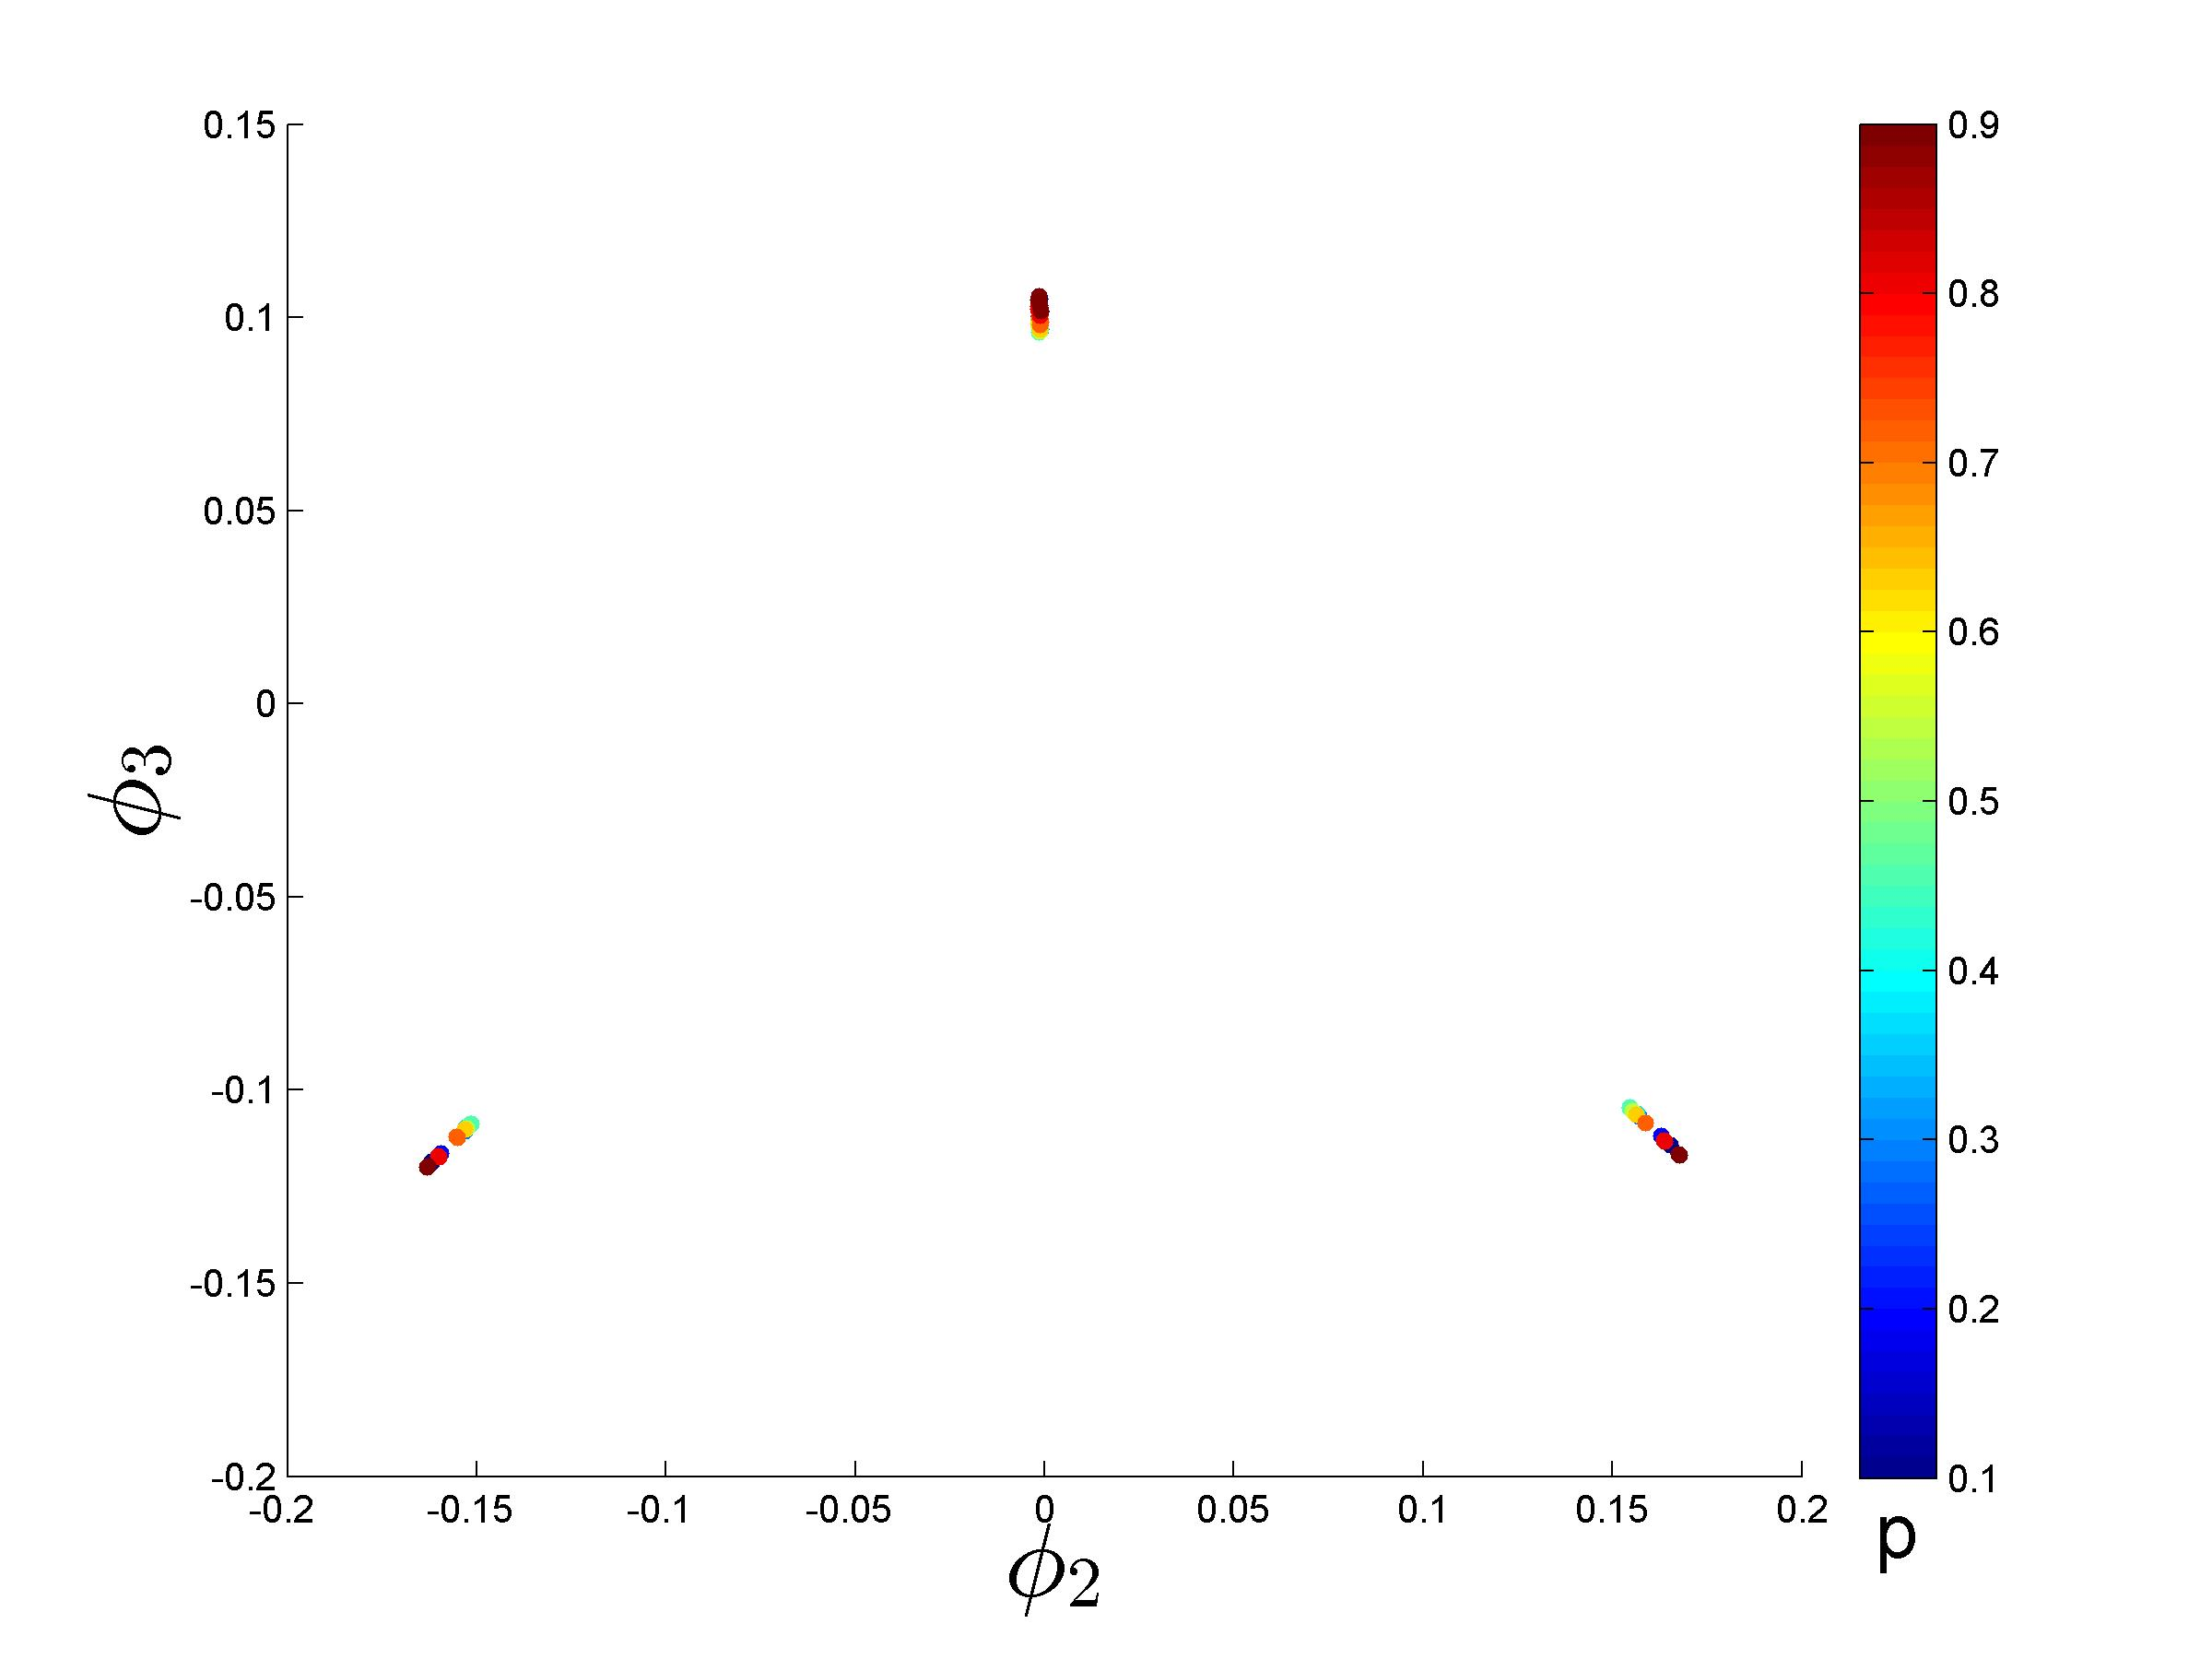
\includegraphics[width=\textwidth]{rawhist_p_1}
%\caption{}
%\end{subfigure}
%\begin{subfigure}{\figwidth}
%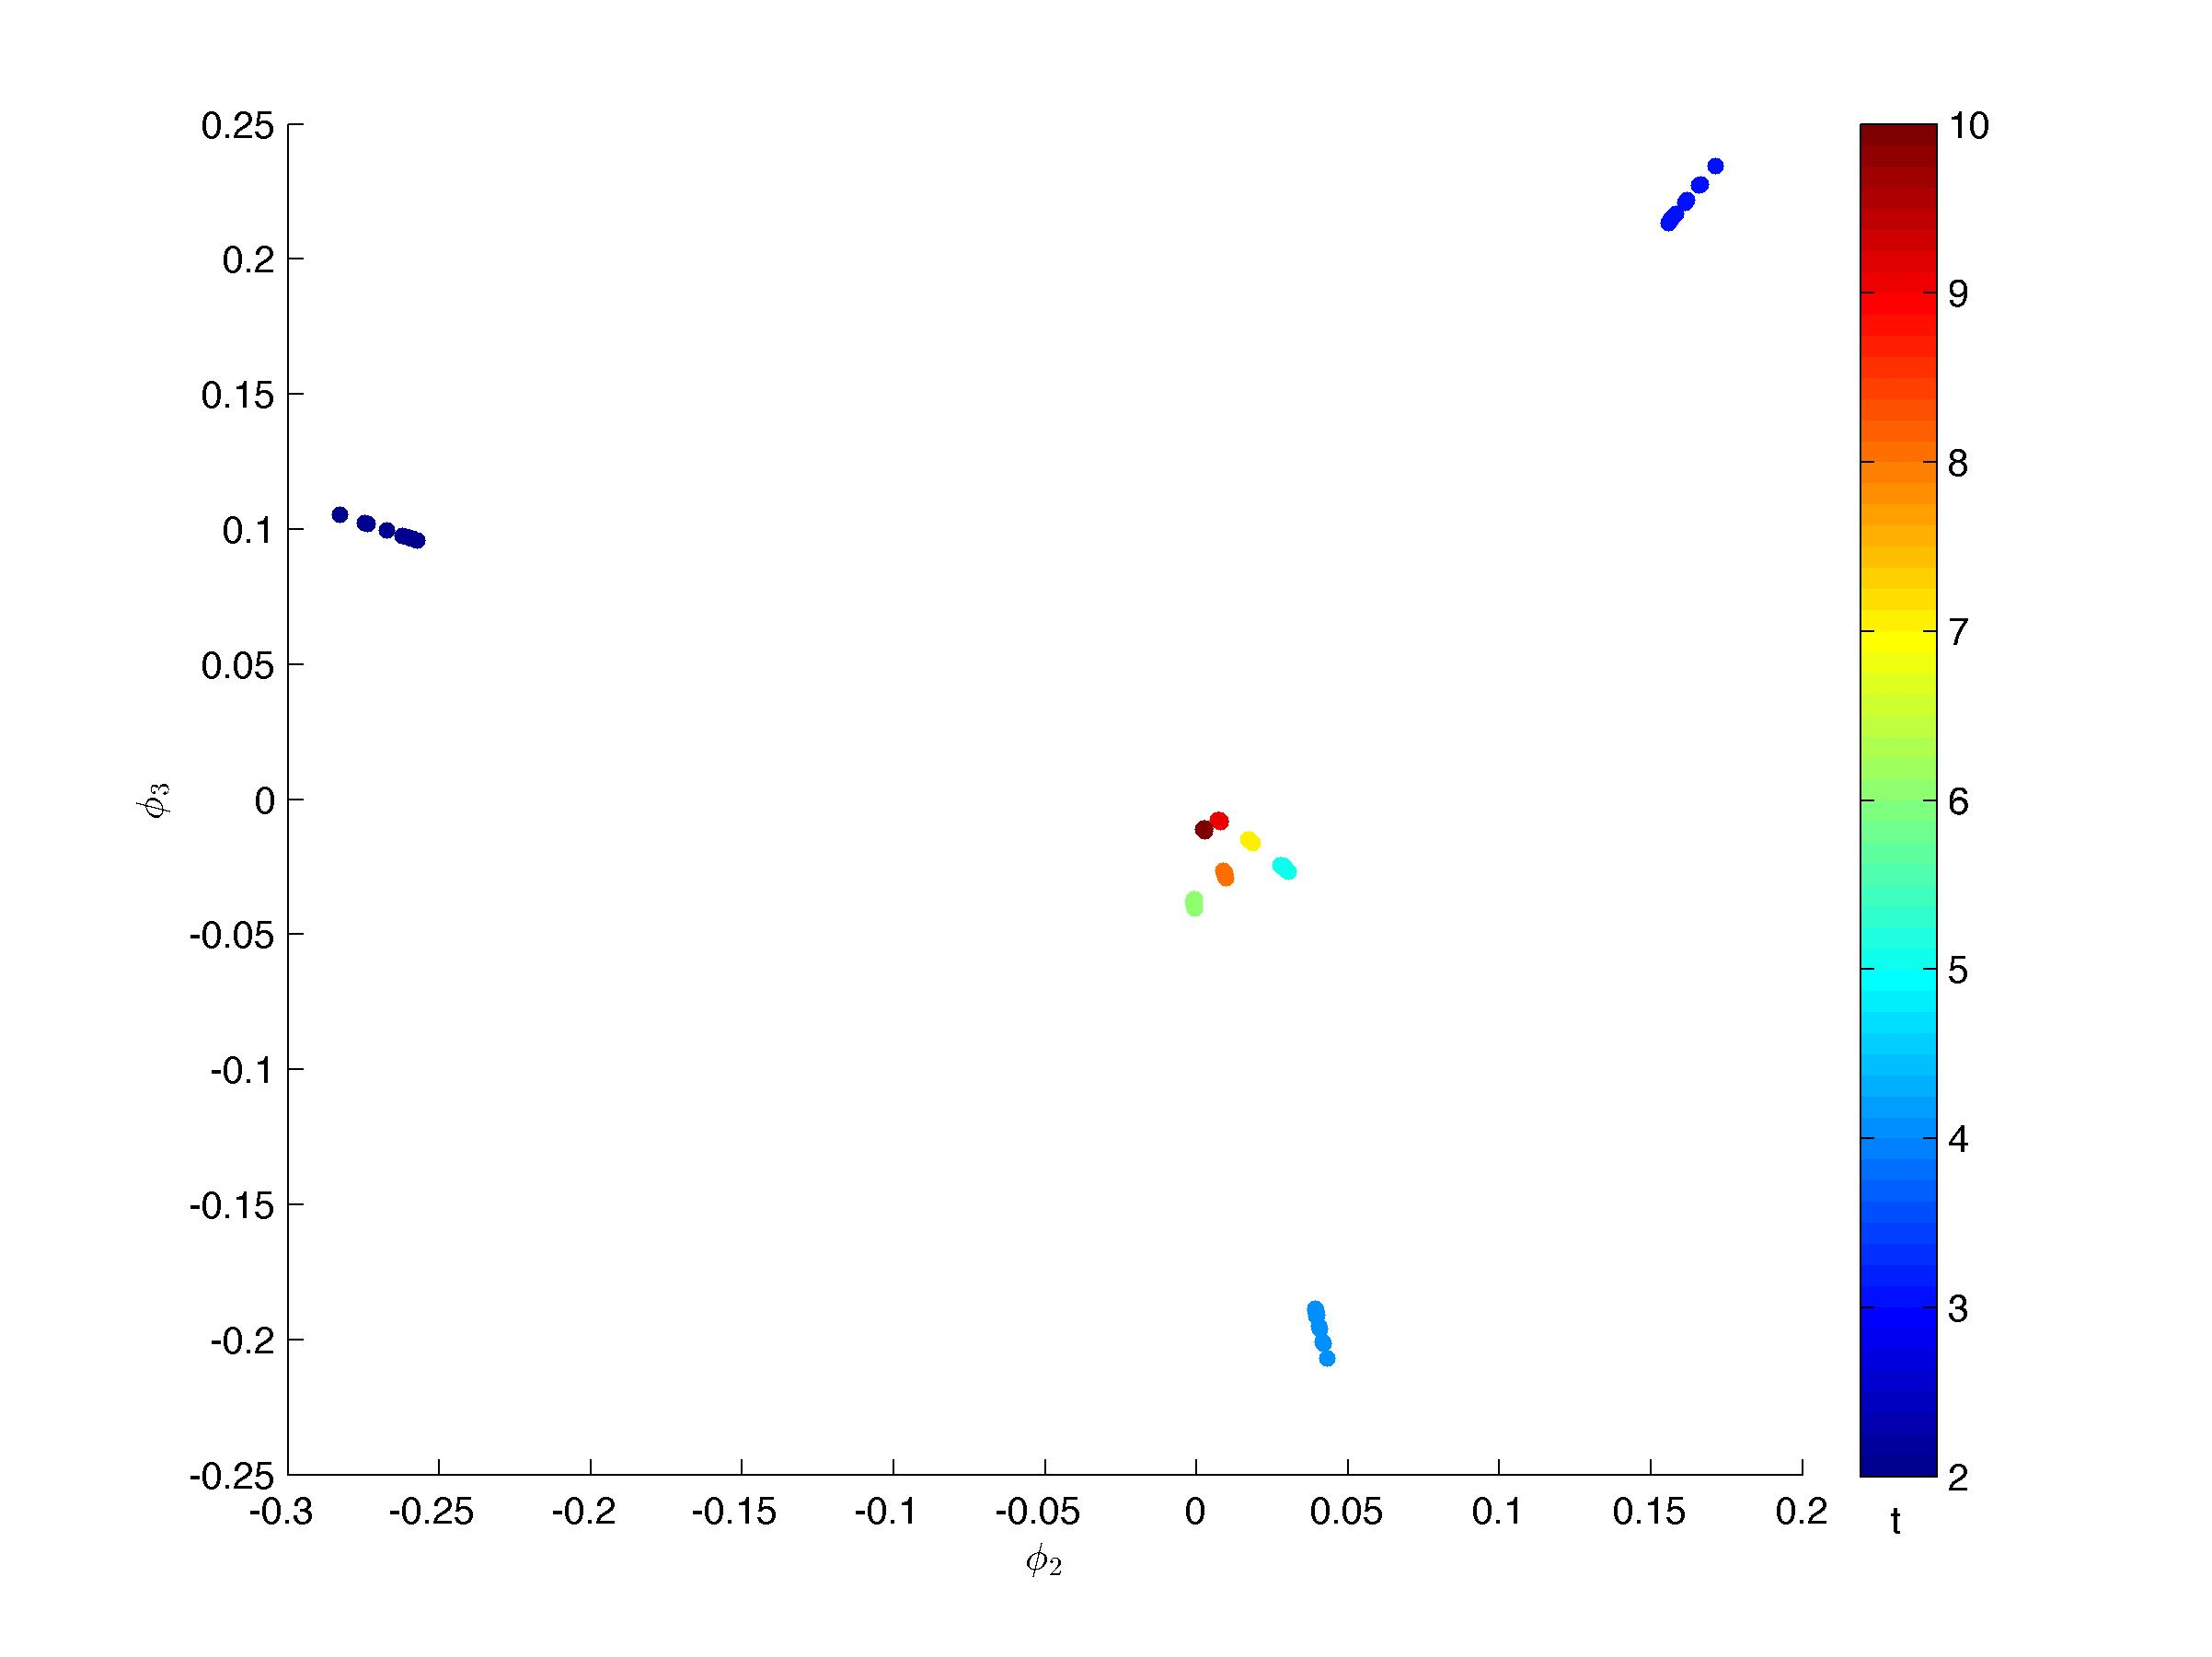
\includegraphics[width=\textwidth]{rawhist_t_1}
%\caption{}
%\end{subfigure}
%\begin{subfigure}{\figwidth}
%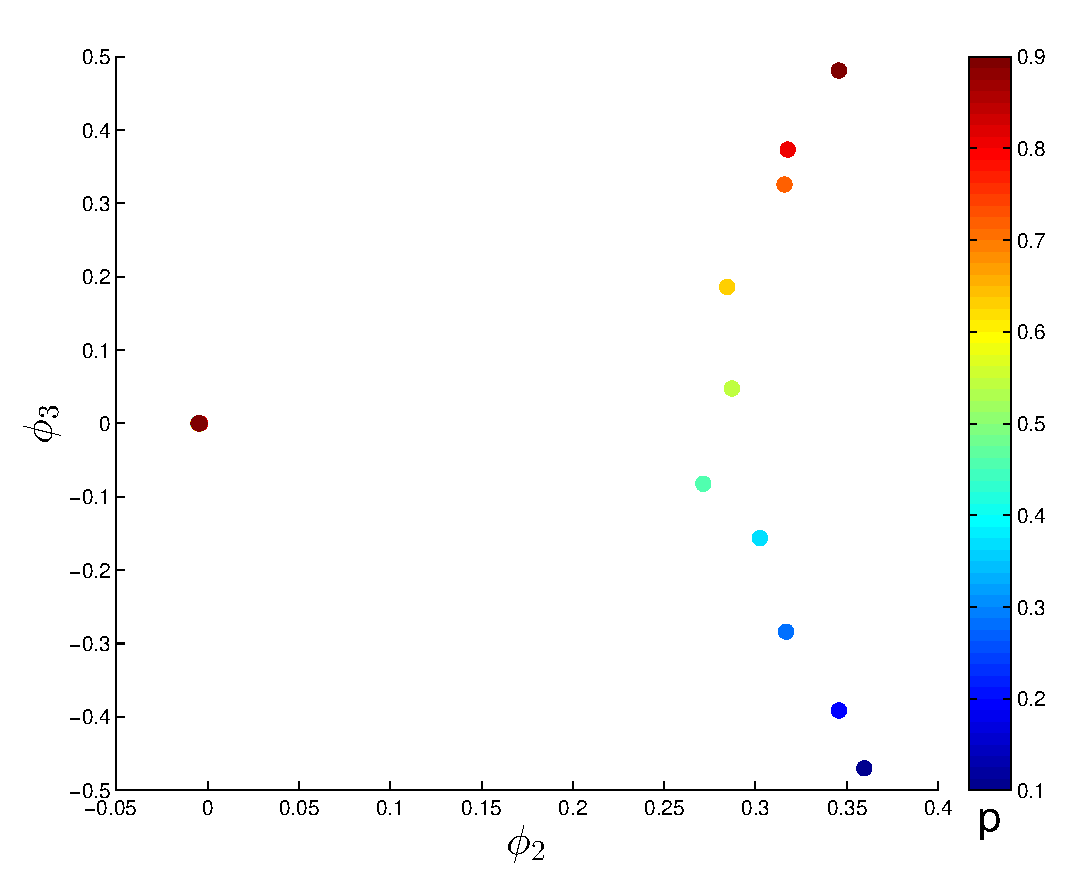
\includegraphics[width=\textwidth]{rawhist_p_400}
%\caption{}
%\end{subfigure}
%\begin{subfigure}{\figwidth}
%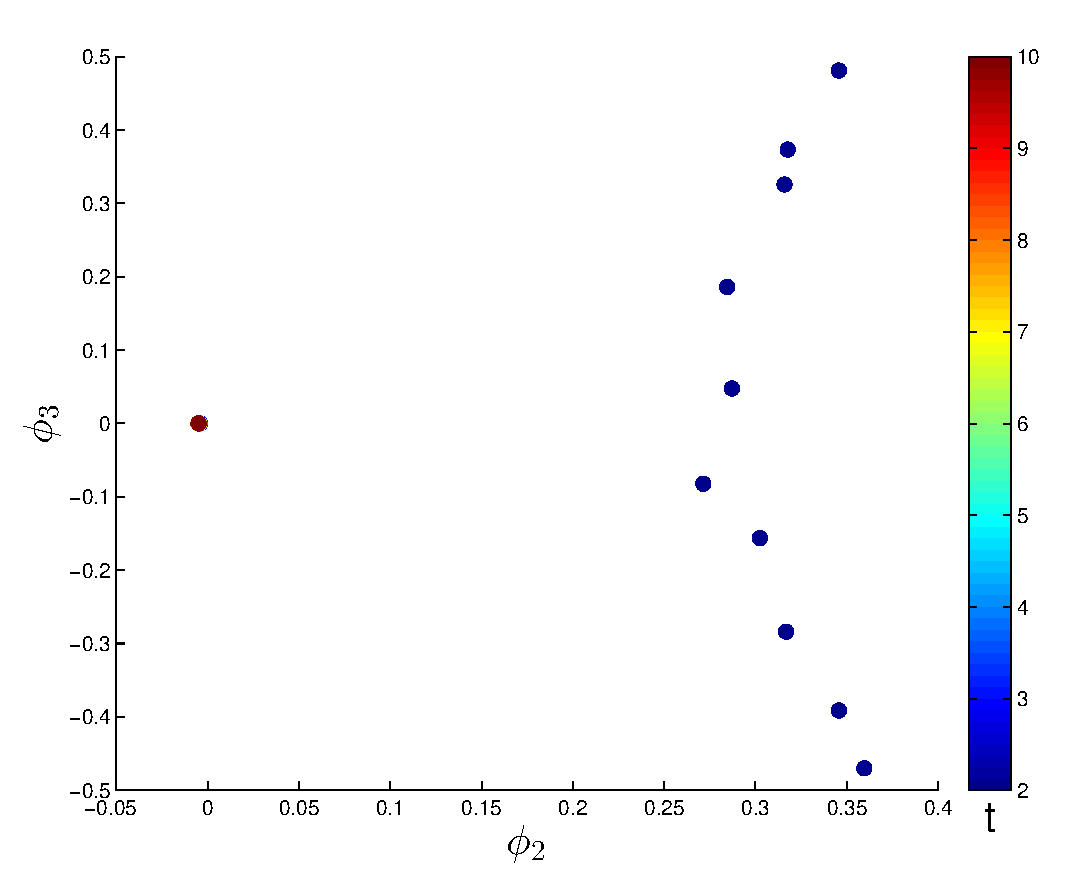
\includegraphics[width=\textwidth]{rawhist_t_400}
%\caption{}
%\end{subfigure}
%\caption{Diffusion maps embeddings computed from simulation data of the velocity jump process with (a,b) $\lambda=1$, $s=1$, and (c,d) $\lambda=400$, $s=20$. The distances used in the diffusion maps kernel are the Euclidean distances between the histograms of particle positions. The data are colored by (a, c) $p$, the initial probability of a particle moving to the right, and (b, d) $t$, time.}
%\label{fig:dmaps_embed_noemd}
%\end{figure}

This paper aims to bridge the fields of data mining and dynamical systems. 
%
For data mining methods to be informative with regards to the underlying system dynamics, processing the appropriate statistical moments or observables instead of individual particles is essential. 
%
In addition, one must also define the appropriate distance metric between the observations.
%
These two components induce the ``correct" Riemannian geometry and allow for informative analyses, such as meaningful and compact parameterization, phase shift detection, and dynamical characterization, through manifold learning.
%
In this paper, these concepts were demonstrated using a dynamical model of cellular chemotaxis with a known macroscopic behavior.
%
We showed that, using histograms as observers and EMD as a distance metric, diffusion maps can uncover a parameterization of the microscale data which is consistent with the analytic macroscopic model.
%
We are confident that such techniques can help inform modeling efforts for systems where the macroscopic dynamics and behavior are not currently known. 

\subsection{Detect dimensionality}


\begin{figure}
%
\def\figheight{1.4in}
%
\begin{subfigure}[t]{0.31\textwidth}
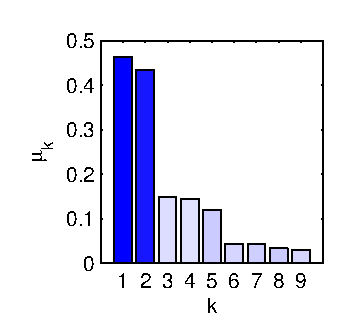
\includegraphics[height=\figheight]{chemotaxis1_evals}
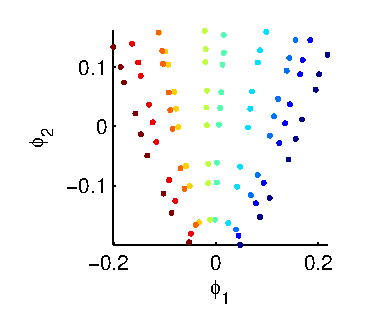
\includegraphics[height=\figheight]{chemotaxis1_embed_good}
%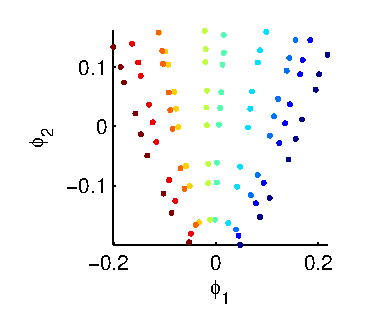
\includegraphics[height=1.5in]{chemotaxis1_embed_bad}
\end{subfigure}
%
\begin{subfigure}[t]{0.31\textwidth}
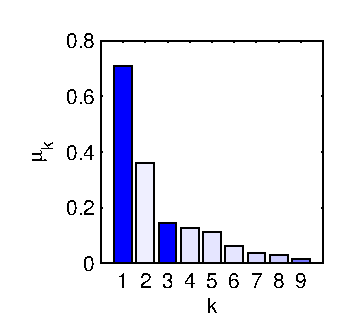
\includegraphics[height=\figheight]{chemotaxis2_evals}
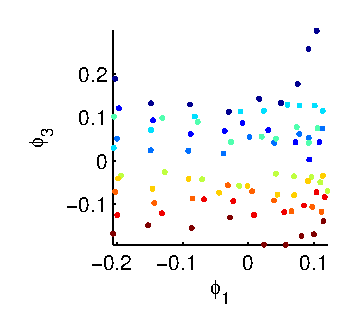
\includegraphics[height=\figheight]{chemotaxis2_embed_good}
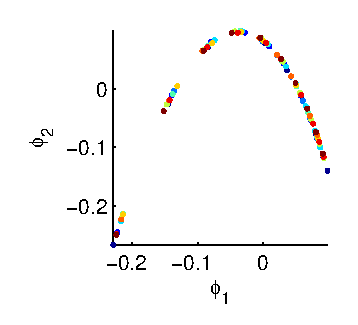
\includegraphics[height=\figheight]{chemotaxis2_embed_bad}
\end{subfigure}
%
\begin{subfigure}[t]{0.35\textwidth}
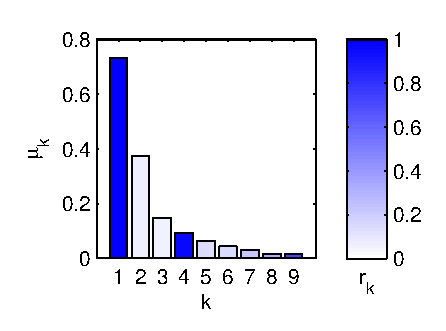
\includegraphics[height=\figheight]{chemotaxis3_evals}
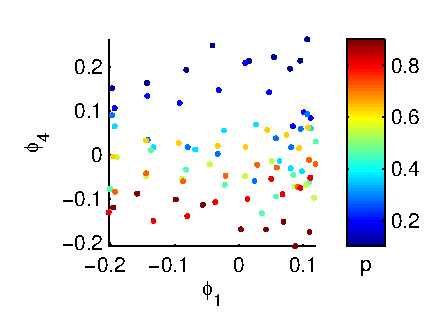
\includegraphics[height=\figheight]{chemotaxis3_embed_good}
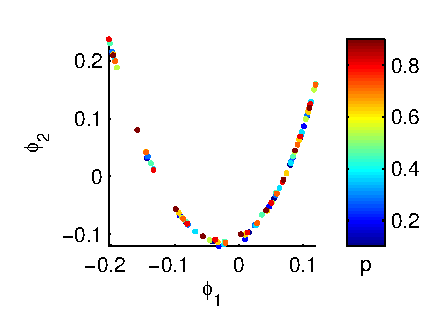
\includegraphics[height=\figheight]{chemotaxis3_embed_bad}
\end{subfigure}
%
\caption{}
%
\end{figure}

\section*{Acknowledgment}
The authors would like to thank TODO.

\bibliographystyle{elsarticle-num}
\bibliography{papers}

\end{document}
